\section{Camera Model}
\subsection{Camera Matrix}
\subsubsection{Pinhole camera model}
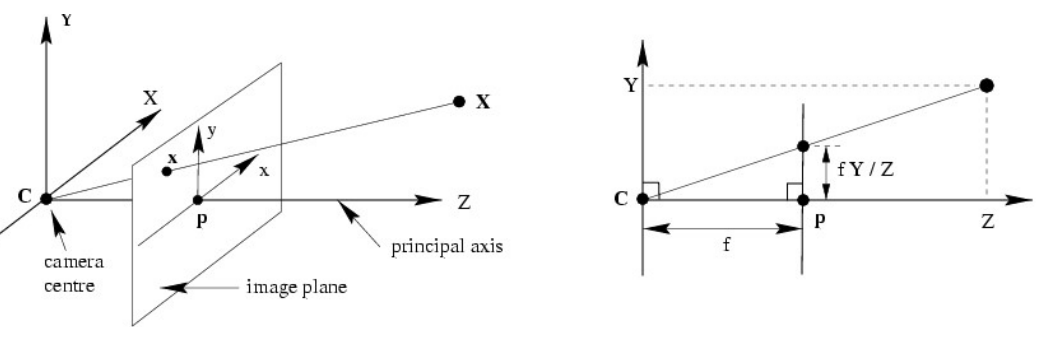
\includegraphics[width=\columnwidth]{pictures/pinholecamera}
Projection on image plane
$$\begin{pmatrix}
fX\\
fY\\
Z\\
\end{pmatrix} = 
\underbrace{\begin{bmatrix}
	f&0&0&0\\
	0&f&0&0\\
	0&0&1&0\\
	\end{bmatrix} }_{= diag(f,f,1)[I|0]} \begin{pmatrix}
X\\
Y\\
Z\\
1\\
\end{pmatrix} $$
By dividing $(fX,fY,Z)^\top$ by $Z$ we get $(x,y,1)^\top$

\subsubsection{Principal Point offset}
Moving the point into the middle of the picture

$$\begin{pmatrix}
fX+Zp_x\\
fY+Zp_y\\
Z\\
\end{pmatrix} = \begin{bmatrix}
f&0&p_x&0\\
0&f&p_y&0\\
0&0&1&0\\
\end{bmatrix} \begin{pmatrix}
X\\
Y\\
Z\\
1\\
\end{pmatrix} $$
By dividing $(fX+Zp_x,fY+Zp_y,Z)^\top$ by $Z$ we get $(x+p_x,y+p_y,1)^\top$

\subsubsection{Kalibration matrix K}
Intrinsic camera parameters

$$ \underbrace{K = \begin{bmatrix}
f&0&p_x\\
0&f&p_y\\
0&0&1\\
\end{bmatrix}}_{simple: a=1 \text{ and } s=0}  \qquad \underbrace{K = \begin{bmatrix}
f&s&p_x\\
0&af&p_y\\
0&0&1\\
\end{bmatrix}}_{general}$$

$f$: focal length\\
$s$: skew between the sensor axes due to the sensor not being mounted perpendicular to the optical axis\\
$a$: aspect ratio between $f_x$ \& $f_y$

\subsubsection{Camera Rotation + Shift}
Extrinsic camera parameters
$$ [R|t] $$
$R$: 3x3 Rotation matrix\\
$t$: 3x1 Translation vector

\subsubsection{Camera Matrix / Projective Camera}
$$ P = K[R|t] $$

$$ \lambda \begin{bmatrix}
u\\
v\\
1\\
\end{bmatrix} = P \begin{bmatrix}
X\\
Y\\
Z\\
W\\
\end{bmatrix} = K[R|t] \begin{bmatrix}
X\\
Y\\
Z\\
W\\
\end{bmatrix} $$

Full matrix has 11 DOF (5 intrinsic +3 rot +3 trans)

3x4 matrix

$$ \tilde{P} = \begin{bmatrix}
K&0\\
0&1\\
\end{bmatrix} \begin{bmatrix}
R&t\\
0^T&1\\
\end{bmatrix} $$
4x4 matrix

$$P = K[R|-RC]$$

\subsection{Camera Calibration with Direct Linear Transform (DLT)}
The DLT method uses a set  of  control  points  whose  object  space/plane  coordinates  are  already  known.  The  control  points  are  normally  fixed  to  a  rigid  frame,  known  as  the  calibration  frame.    The  problem  is  essentially  to  calculate  the  mapping  between  the  2D  image  space  coordinates  (x,y)  and  the  3D  object  space  coordinates  (X,Y,Z).  For this 3D $\leftrightarrow$ 2D correspondence the mapping should take the form of a 3x4 projection matrix (P) such that $x = PX$.

$$ x = PX \rightarrow [x]_xPX = 0 $$

Denoting the rows of $P$ with $P^1, P^2, P^3$ we can rewrite above equation to

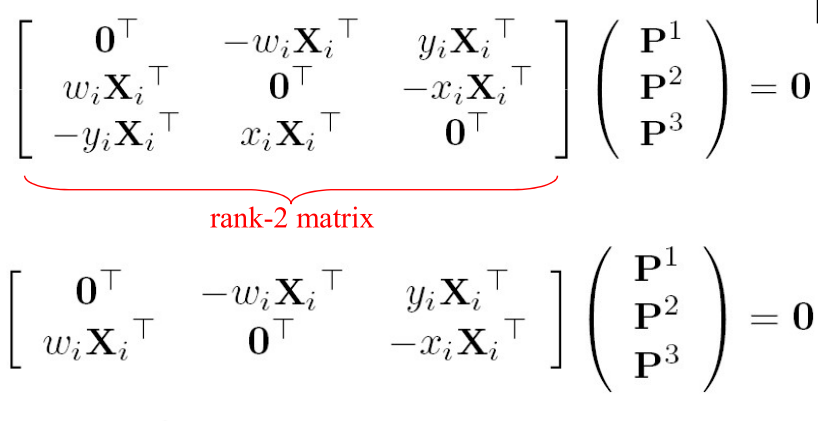
\includegraphics[width=0.7\columnwidth]{pictures/dlt}

Since the third equation is dependant on the first two, it can be discounted. So for every point X we get two equations.

The bracket is denoted with $A$ (2nx12) and the camera matrix with P (3x4)
  
$$ A P = 0 $$

P has 11 DOF $\rightarrow$ 5.5 points are needed for the minimal solution.
For $n \geq 6$ it is over-determined and is solved with SVD.

\subsubsection{Gold Standard algorithm}
Objective:\\
Given $n \geq 6$ 2D to 3D point correspondences, determine the Maximum Likelihood Estimation of the camera projection matrix P.\\

Algorithm:
\begin{enumerate}
	\item Linear Solution: Compute an initial estimate of P using a linear method.
		\begin{enumerate}
			\item Normalization $\tilde{X} = UX$, $\tilde{x} = Tx$
			\item DLT
		\end{enumerate}
	\item Minimization of geometric error: using the linear estimate as a starting point minimize the geometric error: $\min_P \sum_{i}d(\tilde{x}_i,\tilde{P}\tilde{X}_i)^2$
	\item Denormalization $P = T^{-1}\tilde{P}U$
\end{enumerate}